%!TEX root = ../talk.tex

\section{MXNet}\label{sec:MxNet}

%%%

\frameinlbffalse

{
\usebackgroundtemplate{
\tikz[overlay,remember picture] \node[opacity=0.8, xshift=-3.5cm, at=(current page.east)] {

\includegraphics[width=0.35\paperwidth]{figures/mxnet_logo.jpg}
};}

\begin{frame}[plain]
\frametitle{\S\ref{sec:MxNet}. \insertsection}
\listofframes
\end{frame}
\addtocounter{framenumber}{-1} % this page does not count

}

\frameinlbftrue

%%%
\subsection{Programming interface}
%%%

\begin{frame}
  \MyLogo
  \frametitle{General Comments}  

\begin{enumerate}
%
\item Support many different applications (e.g. computer vision, natural language processing,  speech recognition, unsupervised machine learning, support embedded APIs, visualization)
%
\item Mixed programming style: imperative and declarative
\begin{itemize}
\item Light-weighted (around 50K lines of core code)
\item Data parallelism with multi-devices: better scalability
\item Support many front-ends, including JavaScript (run on web browsers)
\item Provide intermediate-level and high-level interface modules
\item Provide abundant IO functions 
%
\end{itemize}
%
\item Fully compatible with Torch: modules and operators
%
\item Visualize neural network graphs
\begin{itemize}
\item Call mx.viz.plot\_network( )
\end{itemize}
%
\item Not well documented, code not easy to read
%
\end{enumerate}

\end{frame}

%%%
\subsection{Simple examples}
%%%

\begin{frame}[fragile]
  \MyLogo
  \frametitle{Example: SoftMax in MXNet}  

\begin{lstlisting}[language=python]
# Fetch the MNIST dataset
import numpy as np
import os, urllib, gzip, struct
def download_data(url, force_download=True): 
	fname = url.split("/")[-1]
	if force_download or not os.path.exists(fname):
		urllib.urlretrieve(url, fname)
	return fname
def read_data(label_url, image_url):
	with gzip.open(download_data(label_url)) as flbl:
		magic, num = struct.unpack(">II", flbl.read(8))
		label = np.fromstring(flbl.read(), dtype=np.int8)
	with gzip.open(download_data(image_url), 'rb') as fimg:
		magic, num, rows, cols = struct.unpack(">IIII", fimg.read(16))
		image = np.fromstring(fimg.read(), dtype=np.uint8).reshape(len(label), rows, cols)
	return (label, image)
path='http://yann.lecun.com/exdb/mnist/'
train_lbl, train_img = read_data(path+'train-labels-idx1-ubyte.gz',
								path+'train-images-idx3-ubyte.gz')
test_lbl, test_img = read_data(path+'t10k-labels-idx1-ubyte.gz',
								path+'t10k-images-idx3-ubyte.gz')
# create data iterators for MXNet
import mxnet as mx
def to4d(img):
	return img.reshape(img.shape[0], 1, 28, 28).astype(np.float32)/255
batch_size = 100
train_iter = mx.io.NDArrayIter(to4d(train_img), train_lbl, batch_size, shuffle=True)
test_iter = mx.io.NDArrayIter(to4d(test_img), test_lbl, batch_size)

\end{lstlisting}

\end{frame}

%%%

\begin{frame}[fragile]
  \MyLogo
  \frametitle{Example: SoftMax in MXNet}  

\ContinueLineNumber
\scriptsize{
\begin{lstlisting}[language=python]
import logging
logging.getLogger().setLevel(logging.INFO)

# A multilayer perceptron contains several fully-connected layers
data = mx.sym.Variable('data') # Create a place holder variable for the input data
data = mx.sym.Flatten(data=data) # Flatten the data from 4-D shape into 2-D

# The first fully-connected layer and according activation function
fc1  = mx.sym.FullyConnected(data=data, name='fc1', num_hidden=128) 
act1 = mx.sym.Activation(data=fc1, name='relu1', act_type="relu")

# The second fully-connected layer and the according activation function
fc2  = mx.sym.FullyConnected(data=act1, name='fc2', num_hidden = 64)
act2 = mx.sym.Activation(data=fc2, name='relu2', act_type="relu")

# The thrid fully-connected layer, note that the hidden size should be 10
fc3  = mx.sym.FullyConnected(data=act2, name='fc3', num_hidden=10)
# The softmax and loss layer
out  = mx.sym.SoftmaxOutput(data=fc3, name='softmax')
mod = mx.mod.Module(out)

# Visualize the network structure with output size
mx.viz.plot_network(symbol=out, shape={'data': (batch_size, 1, 28, 28)}).view()

# Train the model with the above network and data iterators
mod.fit(train_data=train_iter,eval_data=test_iter,num_epoch=10)

\end{lstlisting}
}
%\vskip 100pt
\begin{center}
{\color{red}\scriptsize
https://github.com/dmlc/mxnet/blob/master/example/svm\_mnist/svm\_mnist.py
}
\end{center}

\end{frame}


%%%
\subsection{Visualization}
%%%

\begin{frame}
	\MyLogo
	\frametitle{Graph for example of SoftMax in MXNet}  
	
	\begin{figure}[htbp] 
		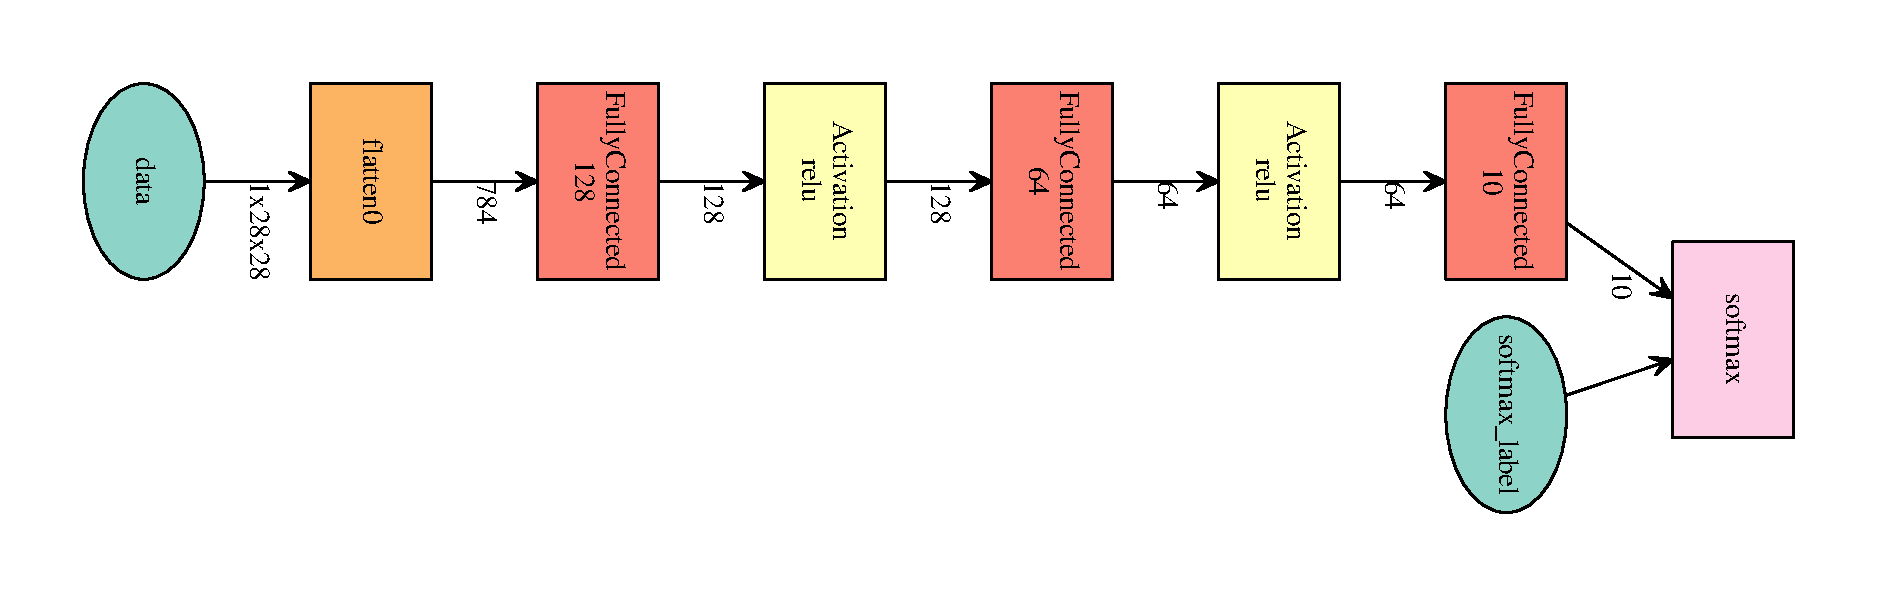
\includegraphics[width=\linewidth]{figures/mxnet_graph.pdf} 
	\end{figure}
	
\end{frame}